\documentclass{beamer}
\mode<presentation>
{
  \usetheme{default}      % or try Darmstadt, Madrid, Warsaw, ...
  \usecolortheme{default} % or try albatross, beaver, crane, ...
  \usefonttheme{default}  % or try serif, structurebold, ...
  \setbeamertemplate{navigation symbols}{}
  \setbeamertemplate{caption}[numbered]
} 

\usepackage[english]{babel}
\usepackage[utf8x]{inputenc}
\usepackage{scrextend}
\usepackage{graphicx}
\usepackage{booktabs}
\usepackage{adjustbox}
\usepackage{marvosym}
\graphicspath{ {E:/faculta/Master/DissertationProject/images/} }

\title[Pres]{Dezvoltarea de metode de analiza automata a sistemelor software}
\author{Student : Stana Adelina Diana}
\author{Conducător stiințific :  prof.dr.ing. Vladimir Crețu}
\institute{Computer Science and Engineering Department\\
"Politehnica" University of Timisoara}
\date{Iulie, 2018}

\begin{document}

\begin{frame}
  \titlepage
\end{frame}

% Uncomment these lines for an automatically generated outline.
%\begin{frame}{Outline}
%  \tableofcontents
%\end{frame}
%%%%%%%%%%%%%%%%%%%%%%%%%%%%%%%%%%%%%%%%%%
 \begin{frame}
\frametitle{Direcțiile și intențiile de studiu avute în vedere pentru programul doctoral}
În cadrul temei de doctorat voi investiga metode de rafinare/filtrare a dependențelor logice extrase din modul de evoluție a sistemelor software, pentru a le putea folosi în aplicații de reconstrucție arhitecturală. Voi investiga în ce măsură utilizarea informațiilor aduse de dependențele logice poate aduce îmbunătățiri metodelor de reconstrucție arhitecturală, atât pentru cele de reclusterizare cât și pentru cele de identificare a modulelor arhitecturale importante.

\end{frame}
%%%%%%%%%%%%%%%%%%%%%%%%%%%%%%%%%%%%%%%%%%

 \begin{frame}
\frametitle{Pregătirea anterioară}

Studiile absolvite pană in prezent sunt:\\
- \textbf{Licența} la facultatea de Automatică și Calculatoare, UPT, in domeniul CTI, specializarea Calculatoare, cu opționale pe pachetul de Software Engineering, media de absolvire 8,87.

Tema lucrarii de licenta a fost \textit{“Sistem distribuit pentru gestionarea interacțiunii clienților cu sistemul de versionare.”} obtinând nota 9,66  în sesiunea Iunie 2016.

- \textbf{Master} la facultatea de Automatică și Calculatoare, UPT, in domeniul CTI, specializarea Information Technology, media de absolvire 9,75. 

Tema lucrarii de dizertatie a fost \textit{“An analysis of the relationship between structural and logical dependencies in software systems.”} obtinând nota 10 în sesiunea Iunie 2018.

\end{frame}

%%%%%%%%%%%%%%%%%%%%%%%%%%%%%%%%%%%%%%%%%%%

 \begin{frame}
\frametitle{Gradul de inițiere în activități de cercetare}
\begin{block}{}
În cadrul departamentului de Calculatoare cu ocazia elaborării lucrării de dizertație. 
\end{block}

Lucrarea de disertație a avut ca obiectiv principal studiul relațiilor dintre diferitele tipuri de dependențe software: dependențe structurale, extrase din analiză statică a codului sursă, și dependențe logice, extrase din modul de evoluție al sistemului regăsit  în sistemul de versionare.
\end{frame}

%%%%%%%%%%%%%%%%%%%%%%%%%%%%%%%%%%%%%%%%%%%

 \begin{frame}
\frametitle{Tool pentru extragerea dependențelor }
S-au studiat 17 sisteme open-source cpp și java. Pentru aceasta, am construit un tool de analiză pentru extragerea ambelor tipuri de dependențe software. 
\begin{center}
     \begin{figure}
	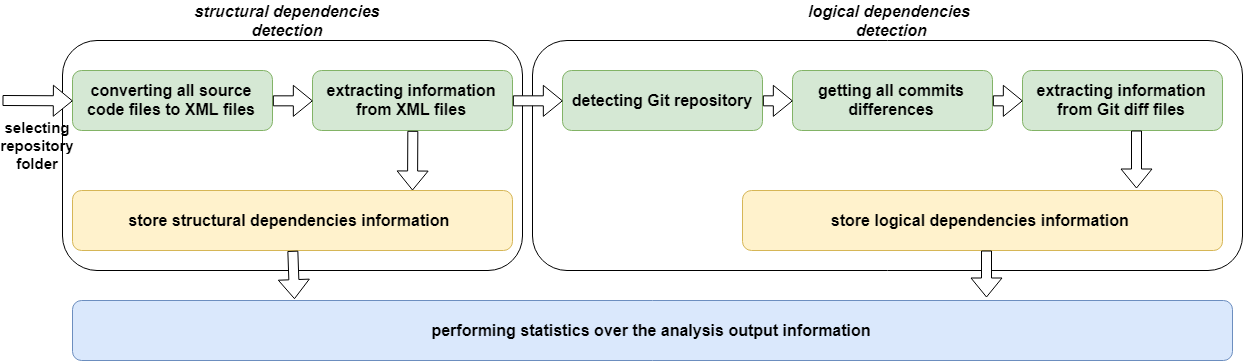
\includegraphics[width=\textwidth]{fig3.png}
	\caption{\label{fig:figtool} Tool workflow}
     \end{figure}
\end{center}

\end{frame}

%%%%%%%%%%%%%%%%%%%%%%%%%%%%%%%%%%%%%%%%%%%

 \begin{frame}
\frametitle{Metode de filtrare ale dependențelor logice}
Dependentele logice au fost extrase în funcție de următoarele filtre :

\begin{itemize}
\item Numărul de fișiere existente într-un commit. Valorile pentru acest filtru: 5, 10, 20 și fără limită de fișiere.
\item Numărul de apariții a unei dependente logice. Valorile pentru acest filtru: 1, 2, 3 și 4 apariții.
\item Cu/fara luarea în considerare a comentariilor ca schimbări valide.
\end{itemize}

\end{frame}

%%%%%%%%%%%%%%%%%%%%%%%%%%%%%%%%%%%%%%%%%%%

 \begin{frame}
\frametitle{Rezultate}

\begin{center}
     \begin{figure}
	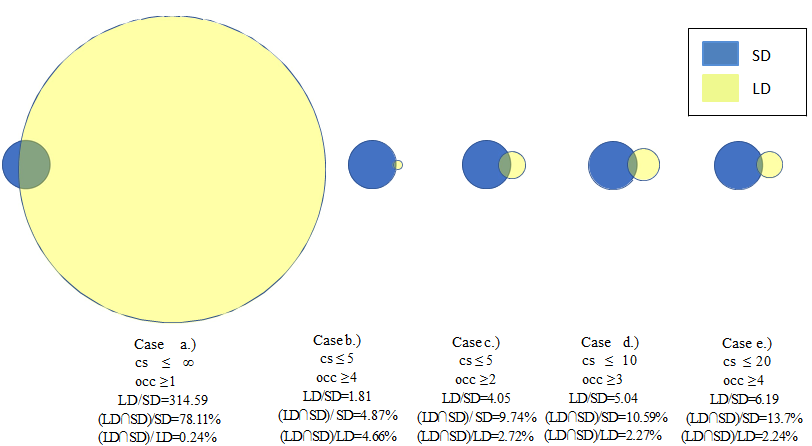
\includegraphics[width=\textwidth]{figvennpdf.png}
	\caption{\label{fig:figvenn} Venn Diagrams}
     \end{figure}
\end{center}


\end{frame}

%%%%%%%%%%%%%%%%%%%%%%%%%%%%%%%%%%%%%%%%%%%

 \begin{frame}
\frametitle{Concluzii preliminare}

\begin{itemize}
\item Cea mai mare influentă asupra rezultatelor o are filtrarea după numărul de fișiere și filtrarea după numărul de apaiții a dependințelor logice 
\item Filtrarea comentariilor are o influentă mică asupra rezultatelor finale.
\end{itemize}

\end{frame}

%%%%%%%%%%%%%%%%%%%%%%%%%%%%%%%%%%%%%%%%%%%

 \begin{frame}
\frametitle{Direcții de continuare a cercetării}


În urma măsuratorilor aproximativ 80\% din dependentele logice nu sunt și structurale. În viitor dorim să studiem cauzele acestei diferențe mari între cele două categorii prin:
\begin{itemize}
\item Extragerea dependentelor structurale și din versiuni mai vechi ale codului, nu doar din cea mai recentă versiune.
\item Filtrarea pe baza trendului crescator sau descrescator in timp al numarului de aparitii al dependentelor logice.
\item Utilizarea informațiilor aduse de dependențele logice în îmbunătățirea metodelor de reconstrucție arhitecturală.
\end{itemize}

\end{frame}

%%%%%%%%%%%%%%%%%%%%%%%%%%%%%%%%%%%%%%%%%%%
 \begin{frame}
\frametitle{Gradul de inițiere în activități practice}
\begin{block}{}
La locul de munca de la Continental(2014-prezent) ca software developer.  Munca mea implică dezvoltare de produse software folosind diferite limbaje de programare: Python, C++, C\# în medii de dezvoltare ca: Visual Studio, PyCharm, folosind diferite sisteme de versionare : SVN, Git.
\end{block}
\end{frame}

%%%%%%%%%%%%%%%%%%%%%%%%%%%%%%%%%%%%%%%%%%%

 \begin{frame}
\frametitle{Lucrări stiințifice}
[1] Adelina Stana, Ioana Șora, \textit{„An analysis of the relationship between structural and logical dependencies in software systems”} trimisă la Sesiunea de Comunicări Ştiinţifice Studenţeşti UPT, comunicată.


[2] Adelina Stana, Ioana Șora, Vladimir Crețu, \textit{„Logical dependencies between classes: how to find them and how to use them ?”} trimisă la The 34th IEEE International Conference on Software Maintenance and Evolution (ICSME) 2018 - Doctoral Symposium, Madrid, Spania, Sept 2018, lucrare acceptată.
\end{frame}

%%%%%%%%%%%%%%%%%%%%%%%%%%%%%%%%%%%%%%%%%%%

 \begin{frame}
\frametitle{Lucrări stiințifice}
[3] Ioana Șora, Adelina Stana, \textit{„Identifying logical dependencies from co-changing classes”}  trimisă la The 7th International Workshop on Mining Software Repositories (SOFTWAREMINING-2018) - colocated with The 33rd IEEE/ACM International  Conference on Automated Software Engineering (ASE 2018), Montpellier, Franta, Sept 2018, în așteptarea deciziei de review.
\end{frame}



%%%%%%%%%%%%%%%%%%%%%%%%%%%%%%%%%%%%%%%%%%%

\end{document}
